\chapter{Планирование траекторий} \label{chapt2}

\section{Введение} \label{sect2_1}
Существует несколько различных ситуаций, в которых требуется планировать траекторию:
\begin{itemize}
	\item Траектория между несколькими точками без избегания препятствий
	\item Траектория между двумя точками без избегания препятствий
	\item Траектория между двумя точками избегающая препятствия
\end{itemize}

Первый случай - результат работы геометрического планировщика, построившего путь с учетом препятствий.
Второй случай является результатом отсутствия геометрического планировщика или быстро изменяющейся динамической среды, в которой находится много перемещающихся препятствий(к примеры многолюдное помещение и тп.п). Третий случай возникает в ситуациях, когда геометрический планировщик построил путь свободный от препятствий или же известно, что они отсутствуют.

Мы не рассматриваем случай генерирования траекторий по нескольким точкам, избегая препятствия, потому что в этом случае путь разбивается на пары точек и используются те же самые методы, что и в траекториях между двумя точками.

\section{Планирование траекторий между несколькими точками без обхода препятствий} \label{sect2_2}
После построения планировщиком пути, необходимо построить траекторию, то есть определить динамические параметры, такие как скорость и ускорение на всем пути. Во-первых нужно получить непрерывный путь, для решения этой задачи можно использовать сплайны. Степень сплайна выбирается исходя из требований к плавности траекторий. В данной работе используются кубические сплайны, которые обеспечивают гладкость функций положения и скорости, а также непрерывность функции ускорения. Функция рывка разрывна, но ограничена сверху и снизу.

\subsection{Интерполяция пути кубическим сплайном} \label{subsect2_2_1}
Каждый полином кубического сплайна имеет четыре коэффициента и представляется в виде: $a_{0}x^{3} + a_{1}x^{2} + a_{2}x + a_{3}$. Из этого следует, что мы можем удовлетворить четыре условия на начальные и конечные значения переменных. Будем считать, что нам известны положения $q_{k},\ q_{k+1}$, а также скорости $v_{k},\ v_{k+1}$ в моменты времени $t_{k}$ и $t_{k+1}$. В таком случае перед нами стоит задача восстановить функцию:
\begin{align*}
	&s(t) = \{q_{k}(t),\ t \in [t_{k}, t_{k+1}],	k=0,\dotsc,n-1\},\\
	&q(k) = a_{k0} + a_{k1}(t - t_{k}) + a_{k2}(t - t_{k})^{2} + a_{k3}(t - t_{k})^{3}
\end{align*}

При это нужно удовлетворить наложенные ограничения:
\begin{align*}
	q_{k}(t_{k}) = q_{k},\ q_{k}(t_{k+1}) = q_{k+1}&,				&\	k=0,\dotsc,n-1\\
	\dot{q}_{k}(t_{k+1}) = \dot{q}_{k+1}(t_{k+1}) = v_{k+1}&,		&\	k=0,\dotsc,n-2\\
	\ddot{q}_{k}(t_{k+1}) = \ddot{q}_{k+1}(t_{k+1})&,				&\	k=0,\dotsc,n-2\\
	\dot{q}_{0}(t_{0}) = v_{0}&,\\
	\dot{q}_{n-1}(t_{n}) = v_{n}&
\end{align*}

Запишем уравнения для k-го полинома, где $T_{k} = t_{k+1} - t_{k}$:
\begin{align*}
	\begin{cases}
		q_{k}(t_{k}) = a_{k0} = q_{k}\\
		\dot{q}_{k}(t_{k}) = a_{k1} = v_{k}\\
		q_{k}(t_{k+1}) = a_{k0} + a_{k1}T_{k} + a_{k2}T_{k}^{2} + a_{k3}T_{k}^{3} = q_{k+1}\\
		\dot{q}_{k}(t_{k+1}) = a_{k1}+ 2a_{k2}T_{k} + 3a_{k3}T_{k}^{2} = v_{k+1}
	\end{cases}
\end{align*}

Разрешая систему относительно неизвестных коэффициентов, получим:
\begin{align*}
	\begin{cases}
		&a_{k0} = q_{k}\\
		&a_{k1} = v_{k}\\
		&a_{k2} = \frac{1}{T_{k}}[\frac{3(q_{k+1} - q_{k})}{T_{k}} - 2v_{k} - v_{k+1}]\\
		&a_{k3} = \frac{1}{T_{k}^2}[\frac{2(q_{k} - q_{k+1})}{T_{k}} + v_{k} + v_{k+1}]
	\end{cases}
\end{align*}

Для решения полученной системы необходимо знать скорости в промежуточных точках, которые мы пока что не знаем. Воспользуемся условиями непрерывности ускорений:
\begin{align*}
	\ddot{q}_{k}(t_{k+1}) = \ddot{q}_{k+1}(t_{k+1}),		&\		k=0,\dotsc,n-2\\
	\ddot{q}_{k}(t_{k+1}) = 2a_{k,2} + 6a_{k,3}T_{k},		&\		k=0,\dotsc,n-2\\
	\ddot{q}_{k+1}(t_{k+1}) = 2a_{k+1,2},					&\		k=0,\dotsc,n-2\\
\end{align*}

Исходя из этих условий, а также принимая во внимание уравнения параметров $a_{k,2}$, $a_{k,3}$ и $a_{k+1,2}$, после нехитрых математических операций и умножения на $\frac{T_{k}T_{k+1}}{2}$ получим следующее выражение:
\begin{align*}
	T_{k+1}v_{k} + 2(T_{k+1}+T{k})v_{k+1} + T_{k}v_{k+2} &= \frac{3}{T_{k}T_{k+1}}[T_{k}^{2}(q_{k+2} - q_{k+1}) + T_{k+1}^{2}(q_{k+1} - q_{k})],\\
	&k=0,\dotsc,n-2
\end{align*}

Эти же выражения можно записать в матричной форме $Av = c$, где:
\begin{align*}
	&A = 
	\begin{bmatrix}
		2(T_{0} + T_{1})	&	T_{0}			&		0	&	\dotsm	&							&						&	0\\
		T_{2}				&	2(T_{2} + T{1})	&	T_{1}	&			&							&						&	0\\
		\vdots				&					&			& 	\ddots	&							&						&	0\\
							&					&			&	T_{n-2}	&	2(T_{n-3} + T_{n-2})	&	T_{n-3}				&	0\\
		0					&			\dotsm	&			&		0	&	T_{n-1}					& 2(T_{n-3} + T_{n-2})	&	T_{n-1}\\
	\end{bmatrix},
\\
	&c =
	\begin{pmatrix}
		\frac{3}{T_{0}T_{1}}[T_{0}^{2}(q_{2} - q_{1}) + T_{1}^{2}(q_{1} - q_{0})] - T_{1}v_{0},\\
		\frac{3}{T_{1}T_{2}}[T_{1}^{2}(q_{3} - q_{2}) + T_{2}^{2}(q_{2} - q_{1})]\\
		\vdots	\\
		\frac{3}{T_{n-3}T_{n-2}}[T_{n-2}^{2}(q_{n-1} - q_{n-2}) + T_{n-2}^{2}(q_{n-2} - q_{n-3})]\\
		\frac{3}{T_{n-2}T_{n-1}}[T_{n-1}^{2}(q_{n} - q_{n-1}) + T_{n-1}^{2}(q_{n-1} - q_{n-2}) - T_{n-2}v_{n}] 
	\end{pmatrix},
\\
	&v =
	\begin{pmatrix}
		v_{1}	&	v_{2}	&	\dotsm	&	v_{n-2}	&	v_{n-1}
	\end{pmatrix}^\mathsf{T}
\end{align*}

Переменные $v_{0}$ и $v_{n}$ исключены из уравнений, поскольку уже известны. Матрица $A$ обладает свойством строгого диагонального преобладания\cite{DDMWiki}, а следовательно всегда обратима. Это означает, что мы всегда можем вычислить значения скоростей в промежуточных точках: $v = A^{-1}c$. После этого вычислить коэффициенты полиномов не составляет труда.


\subsection{Параметризация траектории} \label{subsect2_2_2}
После интерполяции пути тем или иным способом все еще требуется удовлетворить ограничениям на максимальные и минимальные значения производных. Кроме того, хотелось бы, чтобы траектория была оптимальной во времени.

Предположим, что наш полином зависит не от времени, а от параметра $u$. Пусть $u$ - функция времени вида $u(t) = \lambda t$. Тогда:
\begin{align*}
	&\dot{p}(u) = \frac{dp}{du}\frac{du}{dt} = \frac{dp}{du}\lambda \\
	&\ddot{p}(u) = \frac{d^{2}u}{dt^{2}}(\frac{du}{dt})^{2} = \frac{d^{2}u}{dt^{2}}\lambda^{2}\\
	&\dotso
\end{align*}

В этом случае, чтобы удовлетворить наложенным ограничениям и обеспечить оптимальность траектории выберем $\lambda$ как:
\begin{align*}
	\lambda = min(\frac{v_{max}}{p_{max}^{1}(u)},\ \frac{a_{max}}{\sqrt{p_{max}^{2}(u)}}, \frac{j_{max}}{\sqrt[3]{p_{max}^{3}(u)}}, \dots)   
\end{align*}

После параметризации сплайна он уже зависит от времени, участки соответствующие его полиномам можно легко пересчитать по формуле:
\[
	t_{k} = u_{k} / \lambda
\]

\subsection{Результаты} \label{subsect2_2_3}
Для примера возьмем следующую траекторию с двумя степенями свободы. Поскольку время прохождения каждой точки совпадает для траекторий для каждой степени свободы, то траектории автоматически синхронизированы во времени.

\begin{align*}
	&t = \{0, 5, 7, 8, 10, 15, 18\},\\
	&q = \{\{3, -2, -5, 0, 6, 12, 8\},\ \{-5, -2, -3, 0, 5, 8, 15\}\},\\
	&v0 = \{2, 0\},\ v1 = \{-3, 0\}\\
	&v_{max} = 10,\ a_{max} = 15,\ j_{max} = 5
\end{align*}

Результат интерполяции и параметризации представлен на рисунке ниже:
\begin{figure}[ht]
	\centering
	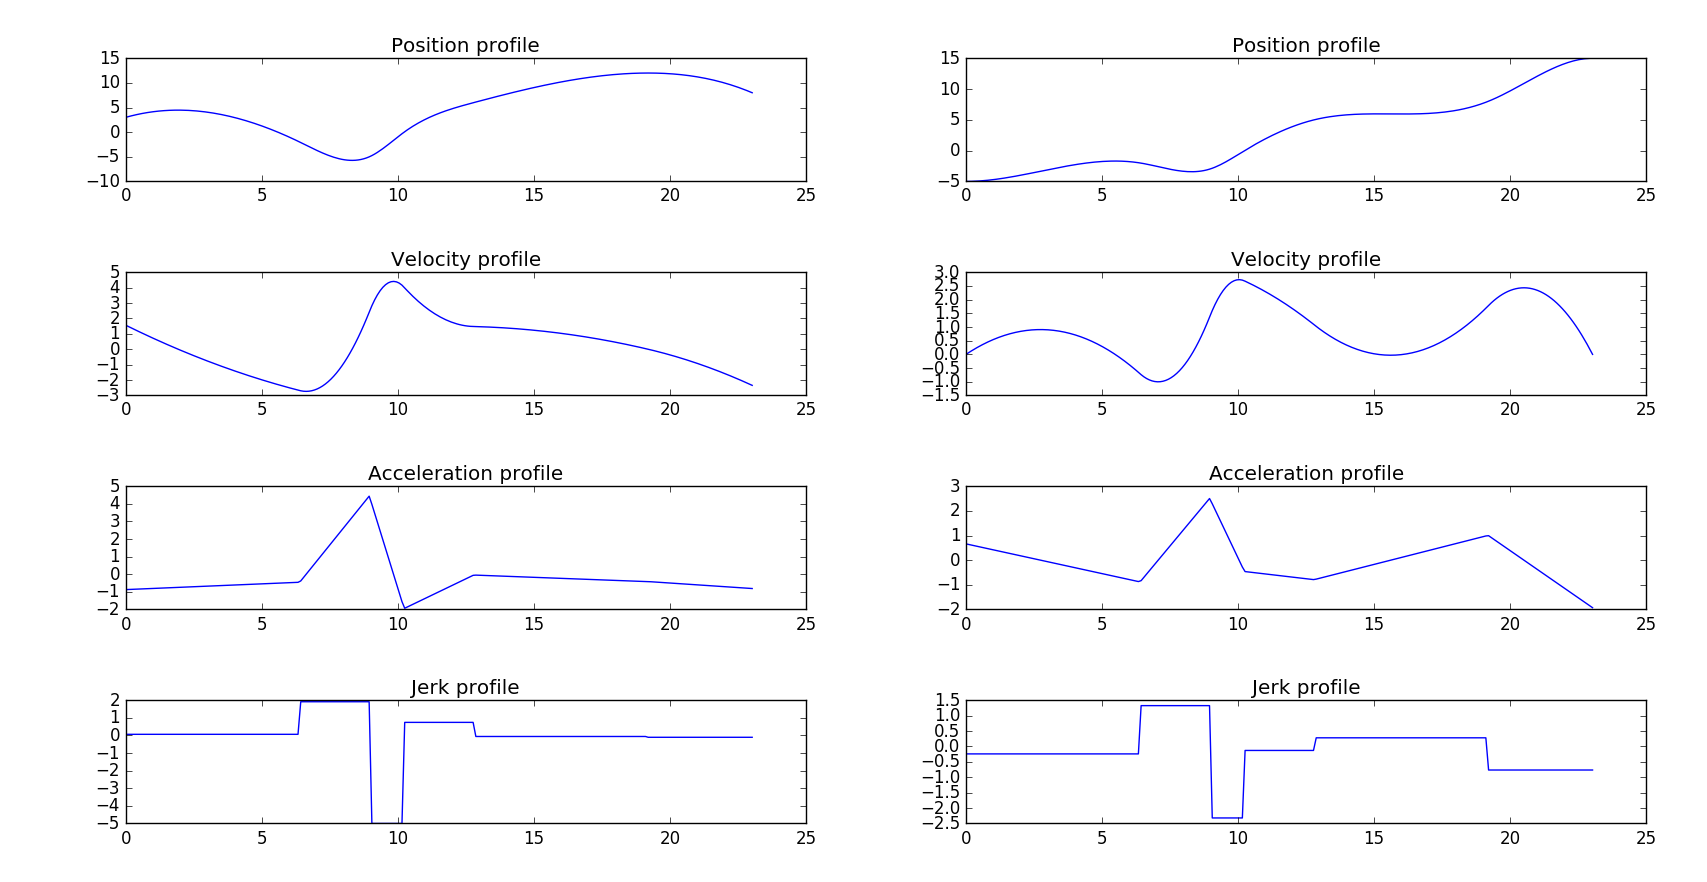
\includegraphics[scale=0.35]{TrajectoryPlanning/cubic_multipoint}
	\caption{Интерполяция и параметризация траектории от времени}
\end{figure}

Как видно из рисунка, данный метод не обеспечивает непрерывности ускорений в начале и в конце движения, что может быть неприемлемо в некторых задачах. В этом случае можно интерполировать всю траекторию или же только первый и последний участок полиномами пятой степени.


\section{Планирование траекторий между двумя точками} \label{sect2_3}

\subsection{Планирование без обхода препятствий} \label{subsect2_3_1}
	Существует огромное количество способов спланировать траекторию между двумя точками без обхода препятствий, но мы остановимся на одном из самых популярных выборов для этой задачи - double S-curve траектории, которые обеспечивают гладкость функции положения и скорости, а также непрерывность функции ускорения. Рывок в свою очередь разрывен, но ограничен максимальным значением.

	Ограничения накладываемые на траекторию:
	\[v_{max},\ a_{max},\ j_{max} \]
	Кроме того выбор начальной и конечной скоростей остается за нами, а вот начальные и конечные ускорения равны нулю.
	
	Траектория имеет три фазы:
	\begin{itemize}
		\item Фаза ускорения $t \in [0,T_{a}]$
		\item Фаза максимальной скорости $t \in [T_{a}, T_{a} + T_{v}]$
		\item Фаза замедления $t \in [T_{a} + T_{v}, T]$, где $T = 2T_{a} + T_{v}$
	\end{itemize}

\subsection{Планирование с обходом препятствий}	\label{subsect2_3_2}